%%%%%%%%%%%%%%%%%%%%%%%%%%%%%%%%%%%%%%%%%
% "ModernCV" CV and Cover Letter
% LaTeX Template
% Version 1.11 (19/6/14)
%
% This template has been downloaded from:
% http://www.LaTeXTemplates.com
%
% Original author:
% Xavier Danaux (xdanaux@gmail.com)
%
% License:
% CC BY-NC-SA 3.0 (http://creativecommons.org/licenses/by-nc-sa/3.0/)
%
% Important note:
% This template requires the moderncv.cls and .sty files to be in the same 
% directory as this .tex file. These files provide the resume style and themes 
% used for structuring the document.
%
%%%%%%%%%%%%%%%%%%%%%%%%%%%%%%%%%%%%%%%%%

%----------------------------------------------------------------------------------------
%	PACKAGES AND OTHER DOCUMENT CONFIGURATIONS
%----------------------------------------------------------------------------------------

\documentclass[11pt,a4paper,sans]{moderncv} % Font sizes: 10, 11, or 12; paper sizes: a4paper, letterpaper, a5paper, legalpaper, executivepaper or landscape; font families: sans or roman

\usepackage[utf8]{inputenc}

\usepackage[export]{adjustbox}

\usepackage{multicol}

\moderncvstyle{casual} % CV theme - options include: 'casual' (default), 'classic', 'oldstyle' and 'banking'
\moderncvcolor{blue} % CV color - options include: 'blue' (default), 'orange', 'green', 'red', 'purple', 'grey' and 'black'

\usepackage{color}

\usepackage{lipsum} % Used for inserting dummy 'Lorem ipsum' text into the template

\usepackage[scale=0.90]{geometry} % Reduce document margins
\setlength{\hintscolumnwidth}{4cm} % Uncomment to change the width of the dates column
%\setlength{\makecvtitlenamewidth}{10cm} % For the 'classic' style, uncomment to adjust the width of the space allocated to your name

%----------------------------------------------------------------------------------------
%	NAME AND CONTACT INFORMATION SECTION
%----------------------------------------------------------------------------------------

\firstname{Jayeon} % Your first name
\familyname{Yoo} % Your last name

% All information in this block is optional, comment out any lines you don't need
\title{Curriculum Vitae}
%\address{14, Gonghangdae-ro 57gil, Gangseo-gu, Seoul, Republic of Korea}
%\mobile{+82 10 8635 3011}
%\phone{(000) 111 1112}
%\fax{(000) 111 1113}
%\email{jayeon0724@gmail.com}
%\homepage{staff.org.edu/~jsmith}{staff.org.edu/$\sim$jsmith} % The first argument is the url for the clickable link, the second argument is the url displayed in the template - this allows special characters to be displayed such as the tilde in this example
%\extrainfo{additional information}
%\photo[70pt][0.4pt]{pictures/picture} % The first bracket is the picture height, the second is the thickness of the frame around the picture (0pt for no frame)
%\quote{}

%----------------------------------------------------------------------------------------

\begin{document}

\textit{\Huge{\textcolor{gray}{Curriculum Vitae}}}

\hrulefill
%----------------------------------------------------------------------------------------
%	PERSONAL SECTION
%----------------------------------------------------------------------------------------

\begin{multicols}{2}
  \section{Personal Information}
  \cvitem{Name}{Jayeon Yoo}
  \cvitem{Date of Birth}{\emph{July 24th, 1993}}
  \cvitem{Address}{14, Gonghangdae-ro 57gil, Gangseo-gu, Seoul, Republic of Korea}
  \cvitem{Mobile}{+82 10 8635 3011}
  \cvitem{Email}{jayeon0724@gmail.com}
  \columnbreak
  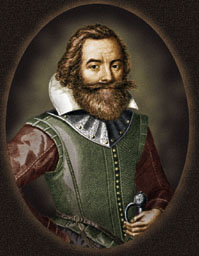
\includegraphics[width=27mm, right]{pictures/picture.jpg}
\end{multicols}

%\section{Presentation}
%\cvitem{}{I'm a Computer Science Engineer with specialization in Software Engineer graduated from Facultat d'Informàtica de Barcelona (UPC). I have 3 years of experience as Java back-end software engineer, both in design/planification and implementation tasks in different international projects at the university, working alongside companies and other universities. I also have some basic experience in front-end development tools. As a freelance developer, I'm currently working in two mobile app projects, and I have some experience in web development as well.}

%----------------------------------------------------------------------------------------
%	EDUCATION SECTION
%----------------------------------------------------------------------------------------

\section{Education}

\cvitem{Mar 2011 -- Aug 2016}{\textbf{Pohang University of Science and Technology   } \textit{Pohang, Korea} \newline B.S. in Industrial Management Engineering}
%\cventry{2008--Present}{Bachelor of Computer Science}{Hanoi University of Science and Technology}{School of Information and Communication Technology, Hanoi.}{\textit{GPA -- 8.0}}{}  % Arguments not required can be left empty

\cvitem{Mar 2009 -- Feb 2011}{\textbf{Hanseong Science High School   } \textit{Seoul, Korea}}


%----------------------------------------------------------------------------------------
%	WORK EXPERIENCE SECTION
%----------------------------------------------------------------------------------------

\section{Work Experience}

\cvitem{Jan 2017 -- Present}{\textbf{Recobell} \textit{Seoul Korea, https://www.recobell.com/   } -- Data Scientist}
\renewcommand{\listitemsymbol}{\textcolor{black}{-~}} % Changes the symbol used for lists
\cvlistitem{Developing item recommendation algorithms running on AWS redshift for various e-commerce service}
\cvlistitem{Analyzing customer’s behaviors and service characteristic for new clients}
\cvlistitem{Reporting the effects of recommendation service and developing the metrics}
\cvlistitem{Research recommendation system}
\subsection{Acheived Projects (Role)}
\renewcommand{\listitemsymbol}{\textcolor{black}{o~}}
\cvlistitem{\textbf{Extracting Representative Keywords of Books} (Independent Data Scientist)
    \newline - Extracting representative nouns of books based on TF-IDF algorithm
    \newline - Making compound nouns from single nouns sets based on Bayesian probability
    \newline - Designing data model for logger
}
\cvlistitem{\textbf{Fraud App Install Detection for CPI Ads} (Assistant Data Scientist)
    \newline - Developing fraud detecting rule sets
    \newline - Feature engineering for decision tree model
}
\cvlistitem{\textbf{Campaign Recommendation for Influencer in a matching platform} (Project Management)
    \newline - Analyzing influencers’ behaviors in platform and distribution of registered campaigns
    \newline - Developing campaign recommendation algorithm based on tag – campaign graph
    \newline - A/B testing and reporting the effects of campaign recommendation
}
\cvlistitem{\textbf{Item Recommendation for O2O service app} (Assistant Data Scientist)
    \newline - Implementation of related item recommendation based on CF
    \newline - Developing item recommendation algorithm for time range and store types
}

\cvitem{Aug 2016 -- Dec 2016}{\textbf{Knowre} \textit{Seoul Korea, http://www.knowre.com/   } -- UX/UI Analyst Intern}
\renewcommand{\listitemsymbol}{\textcolor{black}{-~}} % Changes the symbol used for lists
\cvlistitem{Reporting UX issues of the mathematics education app through the pilot test with students aged 5 -- 7}
\cvlistitem{Designing the process of class using the mathematics education app for learning center}
\cvlistitem{Designing contents of daily and monthly report for parents}
%\renewcommand{\listitemsymbol}{o~} % Changes the symbol used for lists
%\cvlistitem{Project: Making a commercial website using ASP.NET. Finished.}%

%\cventry{12/2013--Present}{Developer}{Bkav Corporation}{Hanoi.}{}{Developed spreadsheets for risk analysis on exotic derivatives on a wide array of commodities (ags, oils, precious and base metals), managed blotter and secondary trades on structured notes, liaised with Middle Office, Sales and Structuring for bookkeeping.
%\newline{}\newline{}
%Detailed achievements:
%\begin{itemize}
%\item Learned how to make amazing coffee
%\item Finally determined the reason for \textsc{PC LOAD LETTER}:
%\begin{itemize}
%\item Paper jam
%\item Software issues:
%\begin{itemize}
%\item Word not sending the correct data to printer
%\item Windows trying to print in letter format
%\end{itemize}
%\item Coffee spilled inside printer
%\end{itemize}
%\item Broke the office record for number of kitten pictures in cubicle
%\end{itemize}}

%------------------------------------------------

%\cventry{2010--2011}{Summer Intern}{\textsc{Lehman Brothers}}{Los Angeles}{}{Rated "truly distinctive" for Analytical Skills and Teamwork.}

%------------------------------------------------

%\subsection{Miscellaneous}

%\cventry{2008--2009}{Computer Repair Specialist}{Buy More}{Burbank}{}{Worked in the Nerd Herd and helped to solve computer problems by asking customers to turn their computers off and on again.}

%----------------------------------------------------------------------------------------
%	EXTRACURRICULAR SECTION
%----------------------------------------------------------------------------------------

\section{Related Activities}

\cvitem{Feb 2019 -- Present}{\textbf{Euler Project} \textit{https://www.hackerrank.com/contests/projecteuler/challenges} \newline - Solving math problem in python}
\cvitem{Oct 2018 -- Dec 2018}{\textbf{Transferring Celebrity’s Make-up to Other Face based on GAN} \newline - Crawling make-up and no make-up face of celebrity from Youtube \newline - Implement MUNIT and LOMIT model}
\

%----------------------------------------------------------------------------------------
%	SKILLS SECTION
%----------------------------------------------------------------------------------------
%\vspace{14mm}
\section{Skills \& Background Knowledge}

\subsection{Technical skills}

\cvitem{}{SQL, \textit{Advanced}}
\cvitem{}{Python, \textit{Advanced}}
\cvitem{}{Spotfire, \textit{Intermediate}}
\cvitem{}{Amazon Web Services (storage and database)}
\cvitem{}{Version control systems (Git)}
\cvitem{}{Agile software development (JIRA)}
\cvitem{}{Basic knowledge of the Linux operating system}



%----------------------------------------------------------------------------------------
%	COMMUNICATION SKILLS SECTION
%----------------------------------------------------------------------------------------

\subsection{Personal skills}

\cvitem{}{High level in communication skills}
\cvitem{}{Sociable and proactive}

%----------------------------------------------------------------------------------------
%	LANGUAGES SECTION
%----------------------------------------------------------------------------------------

\section{Languages}

\cvitem{}{Korean, \textit{Native}}{}
\cvitem{}{English, \textit{Intermediate}}{}
%\cvitem{}{Institutional TOEIC: 570, Hanoi University of Science and Technology, Date taken: 18/8/2013}


%----------------------------------------------------------------------------------------
%	INTERESTS SECTION
%----------------------------------------------------------------------------------------

%\section{Interests}

%\renewcommand{\listitemsymbol}{-~} % Changes the symbol used for lists

%\cvlistitem{Cinema (member of an amateur film production company)}
%\cvlistitem{Acting (member of an amateur theatre company)}

%----------------------------------------------------------------------------------------
%	COVER LETTER
%----------------------------------------------------------------------------------------

% To remove the cover letter, comment out this entire block

%\clearpage

%\recipient{HR Department}{Corporation\\123 Pleasant Lane\\12345 City, State} % Letter recipient
%\date{\today} % Letter date
%\opening{Dear Sir or Madam,} % Opening greeting
%\closing{Sincerely yours,} % Closing phrase
%\enclosure[Attached]{curriculum vit\ae{}} % List of enclosed documents

%\makelettertitle % Print letter title

%\lipsum[1-3] % Dummy text

%\makeletterclosing % Print letter signature

%----------------------------------------------------------------------------------------

\end{document}